\pagestyle{myFancy}
\chapter{Simulations Results}
In this chapter original results from simulations are presented.
The code used to perform such simulations is based on the code originally developed for the calculations presented in refs.~\cite{Panero:2009tv,Mykkanen:2012ri}.

\section{Rotational Invariance Restoration}
This first section has the aim to reproduce the rotational invariance restoration of~\cite{Lang:1982tj} for the continuous group $\SU(2)$ (and not for the discrete icosahedral group $\tilde{Y}$, like explained in \secref{Sec3:RotInv}).
This is done by evaluating the correlator of two Polyakov loops as explained in \secref{Sec2:PolyakovLoops}, computed on two different lattices with two different values of $\beta$, corresponding to two different lattice spacings.
The lattices are taken to be periodic in every direction, with $n_s$ sites in each space direction ($n_s=n_x=n_y=n_z$) and $n_t$ sites in the time direction.\\
The simulations are run from a cold start, with $2500$ thermalization steps, where each Monte Carlo step is composed of $1$ heat bath step followed by $3$ overrelaxation steps.
Since the plaquette is observed to thermalize after $O(10)$ steps in preliminary simulations with both hot and cold starts, $2500$ thermalization steps are enough to ensure full thermalization.\\
After that, $5000$ measurements are taken of every possible independent correlator between two Polyakov loops.
On a lattice with $n_s$ spatial sites in each direction, only couples of Polyakov loops whose distance, in each spatial direction, is $\leq n_s/2$ are independent: for example a couple of Polyakov loops extending for $n_s/2+1$ sites in a certain direction is equivalent to the hermitian conjugate of a couple extending for $n_s/2-1$ sites, because of the periodic boundary conditions (see \eqref{2:nonzeroMomPolyakov}).
But, as the Polyakov loops correlator expectation value is real, they have the same numerical value.\\
In \figref{4F:PolyakovPeriodic} is represented a graphical visualization of this fact.
\begin{figure}[!htbp]
    \centering
    \begin{subfigure}[b]{0.48\textwidth}
        \centering
        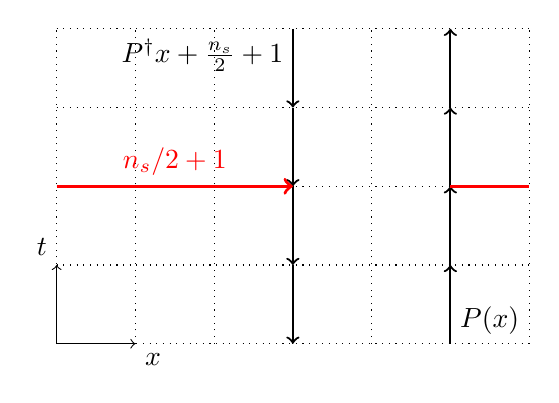
\begin{tikzpicture}
            \draw[step=1.0,dotted] (0,0) grid (6,4);
            \draw[->] (0,0) -- (1,0) node[anchor=north west]{$x$};
            \draw[->] (0,0) -- (0,1) node[anchor=south east]{$t$};
            
            \draw (5,0) node[anchor=south west]{$P(x)$};
            \draw[thick,->] (5,0) -- (5,1);
            \draw[thick,->] (5,1) -- (5,2);
            \draw[thick,->] (5,2) -- (5,3);
            \draw[thick,->] (5,3) -- (5,4);
            
            \draw (3,4) node[anchor=north east]{$P^\dagger\pr{x+\frac{n_s}{2}+1}$};
            \draw[thick,->] (3,4) -- (3,3);
            \draw[thick,->] (3,3) -- (3,2);
            \draw[thick,->] (3,2) -- (3,1);
            \draw[thick,->] (3,1) -- (3,0);
            
            \draw[very thick,red] (5,2) -- (6,2);
            \draw[very thick,red] (1.5,2) node[anchor=south]{$n_s/2+1$};
            \draw[very thick,red,->] (0,2) -- (3,2);
        \end{tikzpicture}
    \end{subfigure}
    \hfill
    \begin{subfigure}[b]{0.48\textwidth}
        \centering
        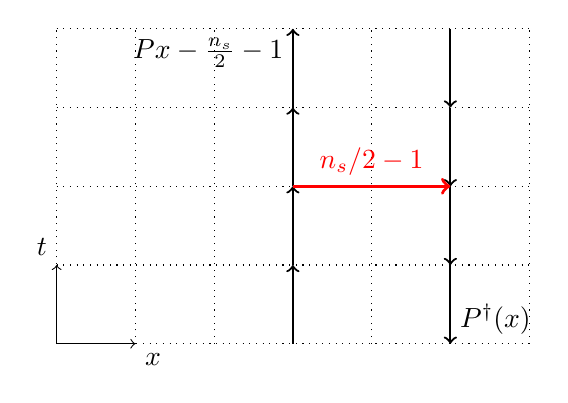
\begin{tikzpicture}
            \draw[step=1.0,dotted] (0,0) grid (6,4);
            \draw[->] (0,0) -- (1,0) node[anchor=north west]{$x$};
            \draw[->] (0,0) -- (0,1) node[anchor=south east]{$t$};
            
            \draw (5,0) node[anchor=south west]{$P^\dagger(x)$};
            \draw[thick,->] (5,4) -- (5,3);
            \draw[thick,->] (5,3) -- (5,2);
            \draw[thick,->] (5,2) -- (5,1);
            \draw[thick,->] (5,1) -- (5,0);
            
            \draw (3,4) node[anchor=north east]{$P\pr{x-\pr{\frac{n_s}{2}-1}}$};
            \draw[thick,->] (3,0) -- (3,1);
            \draw[thick,->] (3,1) -- (3,2);
            \draw[thick,->] (3,2) -- (3,3);
            \draw[thick,->] (3,3) -- (3,4);
            
            \draw[very thick,red,->] (3,2) -- (5,2);
            \draw[very thick,red] (4,2) node[anchor=south]{$n_s/2-1$};
        \end{tikzpicture}
    \end{subfigure}
    \caption{The correlator of two Polyakov loops distant $n_s/2+1$ sites (left) is equal to the hermitian conjugate of the correlator of two Polyakov loops distant $n_s/2-1$ sites (right), \ie $\expval{P(x)P^\dagger\pr{x+\frac{n_s}{2}+1}}=\expval{P^\dagger(x)P\pr{x-\pr{\frac{n_s}{2}-1}}}^\dagger$.}
    \label{4F:PolyakovPeriodic}
\end{figure}\\
Therefore, Polyakov correlators extend only from size $(0,0,0)$ to size $(n_s/2,n_s/2,n_s/2)$.

\section{BCT Lattice Code}
